\chapter{Технологический раздел}


\section{Выбор средств реализации}

\subsection*{Выбор СУБД}


Проведён сравнительный анализ следующих систем управления реляционными базами данных: MySQL~\cite{lit9}, PostgreSQL~\cite{lit10}, Oracle Database~\cite{lit11}, Microsoft SQL Server~\cite{lit12} и SQLite~\cite{lit13}.

Критерии сравнения:
\begin{itemize}
    \item К1 --- бесплатный доступ;
    \item К2 --- поддержка транзакций;
    \item К3 --- поддержка ролевой модели;
\end{itemize}
Результаты анализа представлены в таблице~\ref{tab:dbms_comparison}.


\begin{longtable}{|p{5cm}|C{1cm}|C{1cm}|C{1cm}|}
    \caption{Сравнение СУБД}\label{tab:dbms_comparison} \\
    \hline
    \textbf{СУБД} & \textbf{К1} & \textbf{К2} & \textbf{К3} \\
    \hline
    \endfirsthead
    \multicolumn{4}{l}{\textit{Продолжение таблицы~\ref{tab:dbms_comparison}}} \\
    \hline
    \textbf{СУБД} & \textbf{К1} & \textbf{К2} & \textbf{К3} \\
    \hline
    \endhead
    \endfoot
    \endlastfoot
    MySQL & $+$ & $+$ & $+$ \\
    \hline
    PostgreSQL & $+$ & $+$ & $+$ \\
    \hline
    Oracle Database & $-$ & $+$ & $+$ \\
    \hline
    Microsoft SQL Server & $-$ & $+$ & $+$ \\
    \hline
    SQLite & $+$ & $-$ & $-$ \\
    \hline
\end{longtable}

В результате анализа для разработки выбрана СУБД PostgreSQL, поскольку она соответствует сформулированным критериям.


\section*{Выбор объектного хранилища}

Проведён сравнительный анализ следующих объектных хранилищ: Amazon S3~\cite{lit14}, Google Cloud Storage~\cite{lit15}, MinIO~\cite{lit16}.

Критерии сравнения:
\begin{itemize}
    \item бесплатный доступ;
    \item минимальное потребление ОЗУ;
    \item модель развёртывания.
\end{itemize}
Результаты анализа представлены в таблице~\ref{tab:object_storage_comparison}.

\begin{longtable}{|p{5.5cm}|C{1cm}|C{1cm}|C{2.3cm}|}
    \caption{Сравнение объектных хранилищ}\label{tab:object_storage_comparison} \\
    \hline
    \textbf{Объектное хранилище} & \textbf{К1} & \textbf{К2} & \textbf{К3} \\
    \hline
    \endfirsthead
    \multicolumn{4}{l}{\textit{Продолжение таблицы~\ref{tab:object_storage_comparison}}} \\
    \hline
    \textbf{Объектное хранилище} & \textbf{К1} & \textbf{К2} & \textbf{К3} \\
    \hline
    \endhead
    \endfoot
    \endlastfoot
    Amazon S3 & $-$ & $-$ & облачная \\
    \hline
    Google Cloud Storage & $-$ & $-$ & облачная \\
    \hline
    MinIO & $+$ & $+$ & локальная \\
    \hline
\end{longtable}

В результате анализа для разработки выбрано объектное хранилище MinIO\@.

\subsection*{Выбор средств реализации программного обеспечения}

Для реализации приложения выбран язык программирования Go~\cite{lit17}, поскольку он ориентирован на разработку серверных приложений и обладает набором пакетов для работы с REST API, базами данных и хранилищами.
Разработка будет осуществляться в среде разработки JetBrains GoLand~\cite{lit18}, которая обеспечивает инструменты для написания, отладки и тестирования кода на языке Go\@.


\section{Проектирование программного обеспечения}

При моделировании архитектуры программной системы использован метод графического моделирования C4.
На уровне контейнеров система представлена как связка Web SPA, Backend, базы данных PostgreSQL, кеша Redis и объектного хранилища MinIO\@.
Web SPA взаимодействует с Backend по REST API для операций.
Backend хранит метаданные и бизнес-сущности в PostgreSQL, а загрузка/получение видео выполняется через MinIO с использованием presigned URL, выдаваемых Backend.
Backend использует Redis для кеширования статистики, счётчиков и refresh-сессий, чтобы снизить нагрузку на БД.
Роли пользователей (гость, пользователь, модератор, администратор) отражают сценарии доступа в интерфейсе.

Схема связи компонентов представлена на рисунке~\ref{fig:l2}.
\begin{figure}[H]
    \centering
    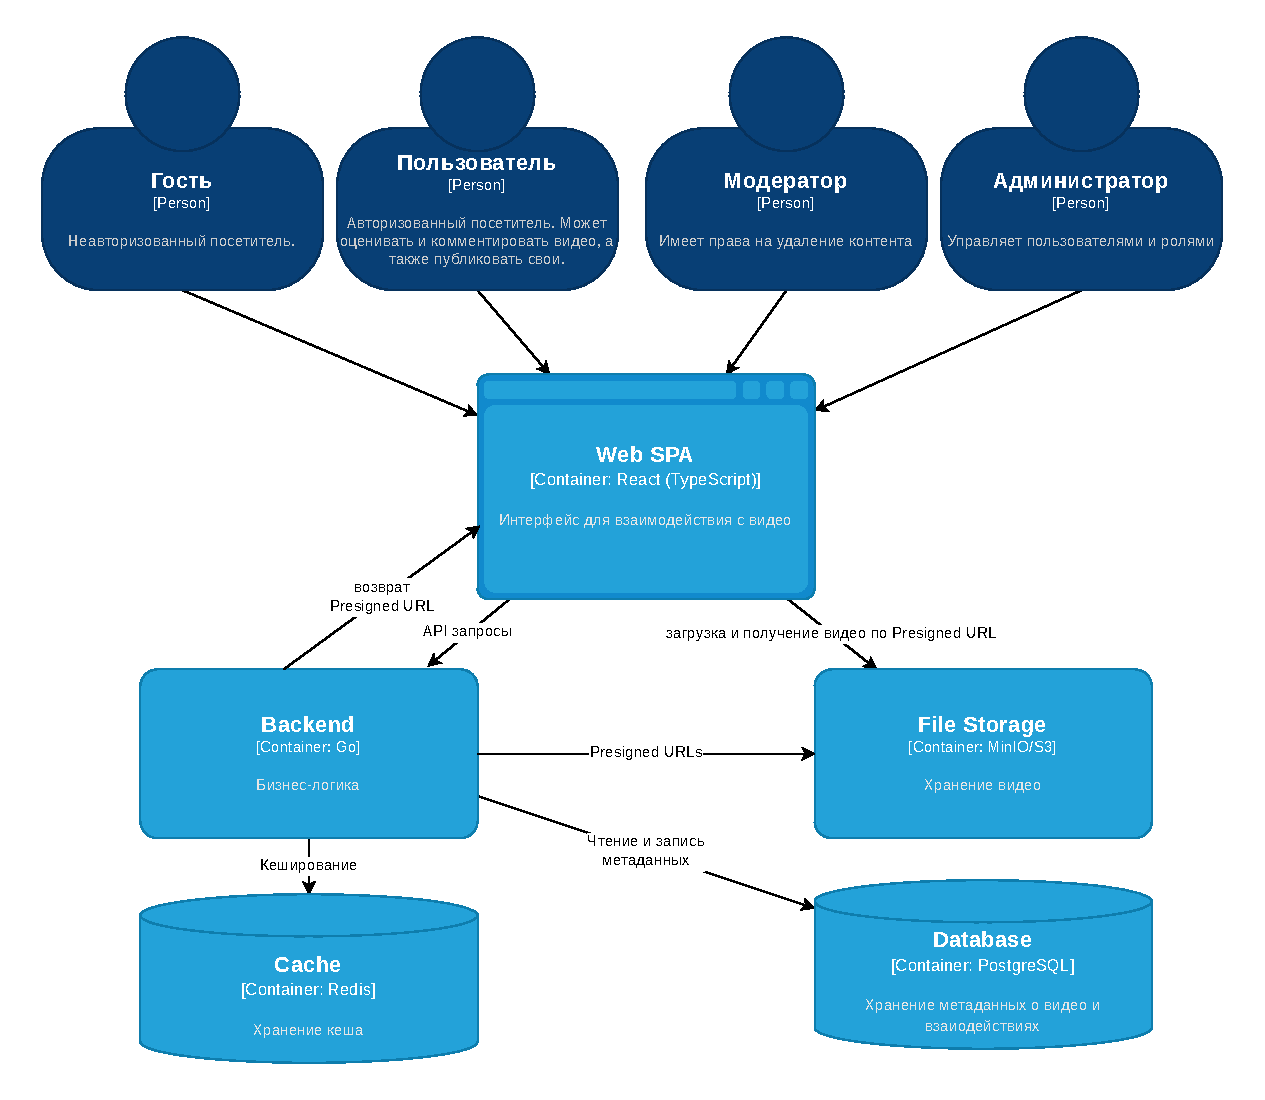
\includegraphics[width=0.7\textwidth]{ppo/C4-L2.drawio}
    \caption{Уровень контейнеров архитектуры системы}
    \label{fig:l2}
\end{figure}

Для уточнения взаимодействия компонентов приведена диаграмма последовательности процесса загрузки видео.
Диаграмма показывает шаги обмена между Web SPA, Backend, PostgreSQL и MinIO, фиксирует порядок вызовов и точки ответственности.
Диаграмма последовательности представлена на рисунке~\ref{fig:sequence_upload_video}.
\begin{figure}[H]
    \centering
    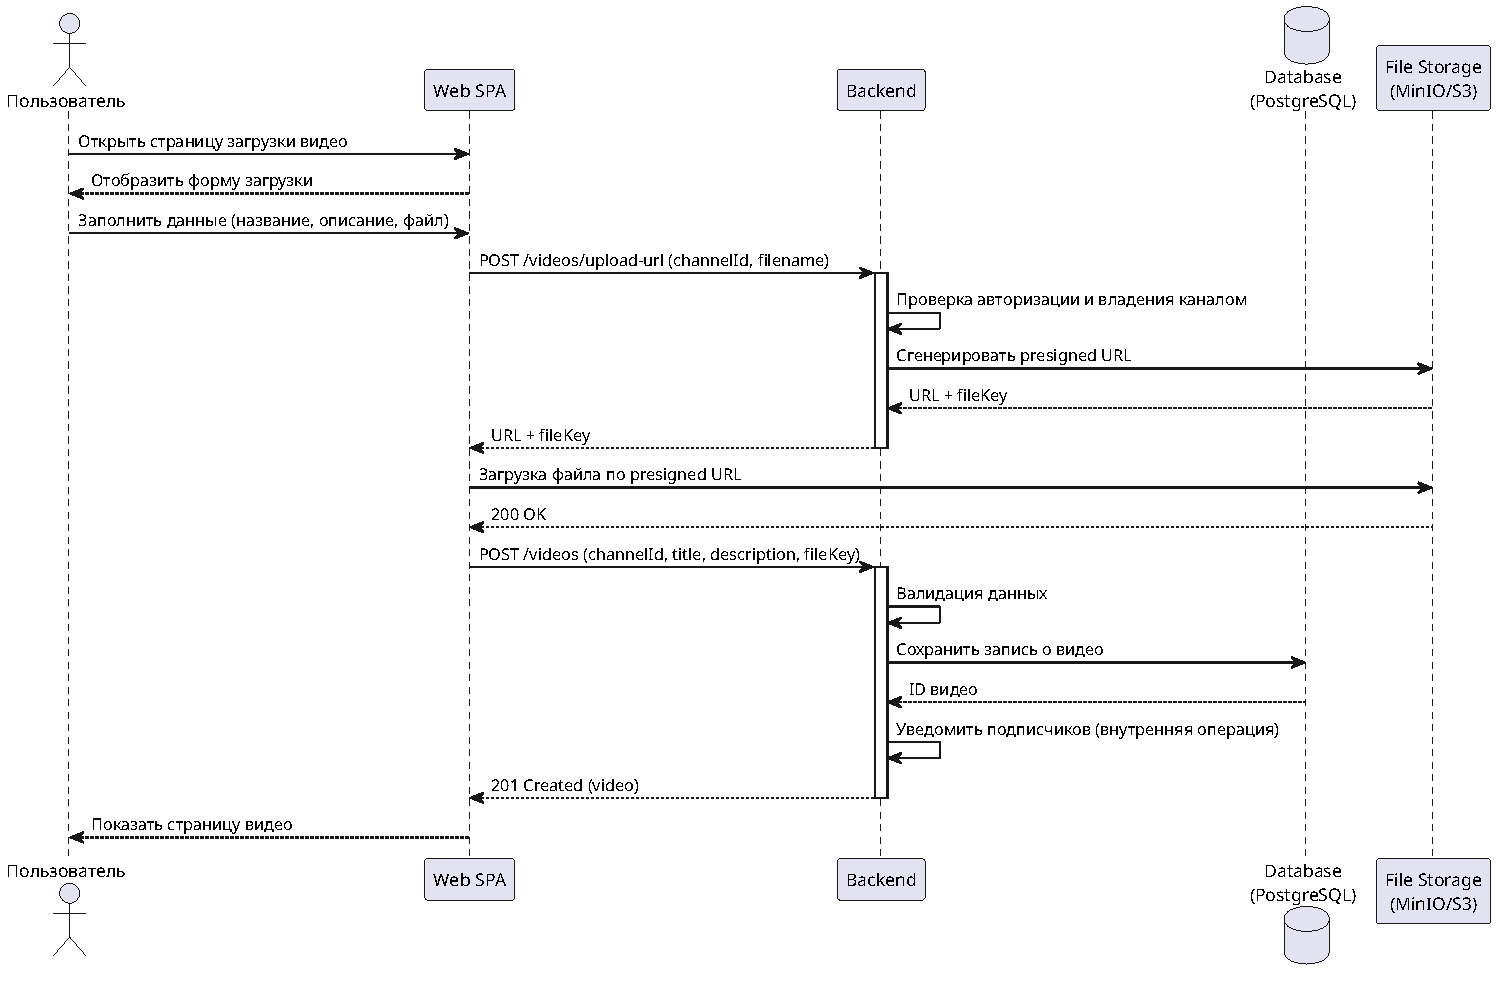
\includegraphics[width=0.7\textwidth]{ppo/sequence_upload_video}
    \caption{Диаграмма последовательности процесса загрузки видео}
    \label{fig:sequence_upload_video}
\end{figure}


\section{Разработка программного обеспечения}

\subsection*{Разработка базы данных и приложения доступа}

База данных реализована в PostgreSQL с использованием миграций, содержащих создание таблиц, и ограничений целостности.
Приложение доступа реализовано в виде REST API, обеспечивающего операции регистрации, публикации видео, управления подписками и взаимодействия с контентом.
Для проверки требований сформирован тестовый набор данных не менее 1000 записей для каждой таблицы.

Сценарий создания базы данных приведён в листинге~\ref{lst:db_schema}.
На стороне СУБД реализована хранимая функция уведомления подписчиков канала о новом видео, которая выполняет обновление счётчиков новых видео только для подписчиков с включёнными уведомлениями.
Реализация функции представлена в листинге~\ref{lst:sql}.

\subsection*{Внешнее кэширование с использованием Redis}

В качестве InMemory СУБД используется Redis для кэширования счётчиков и агрегированной статистики.
Кэш содержит значения просмотров, лайков и дизлайков по видео, а также счётчики новых уведомлений, что снижает нагрузку на базу данных.
При записи новых событий происходит инвалидация и обновление кеша при следущем запросе.


\section{Тестирование программного обеспечения}

Проверка корректности работы выполнялась на двух уровнях: модульном и интеграционном.
Модульные тесты применялись для сервисного слоя, использовались фиктивные реализации внешних зависимостей, что позволило изолировать бизнес-логику.
Интеграционные тесты применялись для слоя репозиториев PostgreSQL\@.
Хранимая процедура PostgreSQL для уведомления подписчиков о новом видео также протестирована интеграционными тестами.

Классы эквивалентности для тестирования хранимой процедуры для уведомления подписчиков представлены в таблице~\ref{tab:sql_eq_classes}.

\begin{longtable}{|p{2.3cm}|p{7cm}|p{5.5cm}|}
    \caption{Классы эквивалентности для хранимой процедуры уведомления подписчиков}\label{tab:sql_eq_classes} \\
    \hline
    \textbf{Параметр} & \textbf{Класс эквивалентности} & \textbf{Ожидаемый результат} \\
    \hline
    \endfirsthead
    \multicolumn{3}{l}{\textit{Продолжение таблицы~\ref{tab:sql_eq_classes}}} \\
    \hline
    \textbf{Параметр} & \textbf{Класс эквивалентности} & \textbf{Ожидаемый результат} \\
    \hline
    \endhead
    \endfoot
    \endlastfoot
    channel\_id & Канал существует, есть подписчики с включёнными уведомлениями & Счётчики новых видео увеличены \\
    \hline
    channel\_id & Канал существует, подписчиков нет & Изменений нет \\
    \hline
    channel\_id & Канал существует, подписчики есть, но уведомления отключены & Изменений нет \\
    \hline
    channel\_id & Канал не существует & Ошибка/отсутствие изменений \\
    \hline
    video\_id & Видео существует и принадлежит каналу & Уведомление формируется \\
    \hline
    video\_id & Видео не существует или не принадлежит каналу & Ошибка/отсутствие изменений \\
    \hline
\end{longtable}

Примеры тестов, используемых при проверке функциональности, представлены в таблице~\ref{tab:test_examples}.

\begin{longtable}{|p{2cm}|p{9cm}|p{4cm}|}
    \caption{Примеры тестов}\label{tab:test_examples} \\
    \hline
    \textbf{№ теста} & \textbf{Описание теста} & \textbf{Ожидаемый результат} \\
    \hline
    \endfirsthead
    \multicolumn{3}{l}{\textit{Продолжение таблицы~\ref{tab:test_examples}}} \\
    \hline
    \textbf{№ теста} & \textbf{Описание теста} & \textbf{Ожидаемый результат} \\
    \hline
    \endhead
    \endfoot
    \endlastfoot
    1 & Регистрация пользователя: проверка создания пользователя с валидными данными и назначением роли по умолчанию. & Пользователь создан, роль назначена. \\
    \hline
    2 & Создание канала: проверка, что канал создаётся только при отсутствии канала у пользователя и уникальном имени. & Канал создан, возвращён идентификатор. \\
    \hline
    3 & Уведомление подписчиков: проверка увеличения счётчика новых видео для подписчиков с включёнными уведомлениями. & Счётчик новых видео увеличен. \\
    \hline
\end{longtable}

Все тесты пройдены успешно.


\section*{Выводы по разделу}

В технологическом разделе обоснован выбор СУБД PostgreSQL, объектного хранилища MinIO и языка Go.
Описана архитектура системы на уровне контейнеров и взаимодействие компонентов.
Приведён подход к тестированию и набор тестовых примеров.
